%!TEX root = notex.tex

\section{Some Information}

\lipsum[0-1]

\begin{equation}
    \vec{E} = - \left( \frac{\partial V}{\partial x} \ \hat{x} + \frac{\partial V}{\partial y} \ \hat{y} + 
    \frac{\partial V}{\partial z} \ \hat{z} \right) = - (\vec{E_{x}} + \vec{E_{y}} + \vec{E_{z}})
\end{equation}

\lipsum[2-3]

\subsection{A subsection}

\lipsum[4-5]

\begin{figure}[h]
    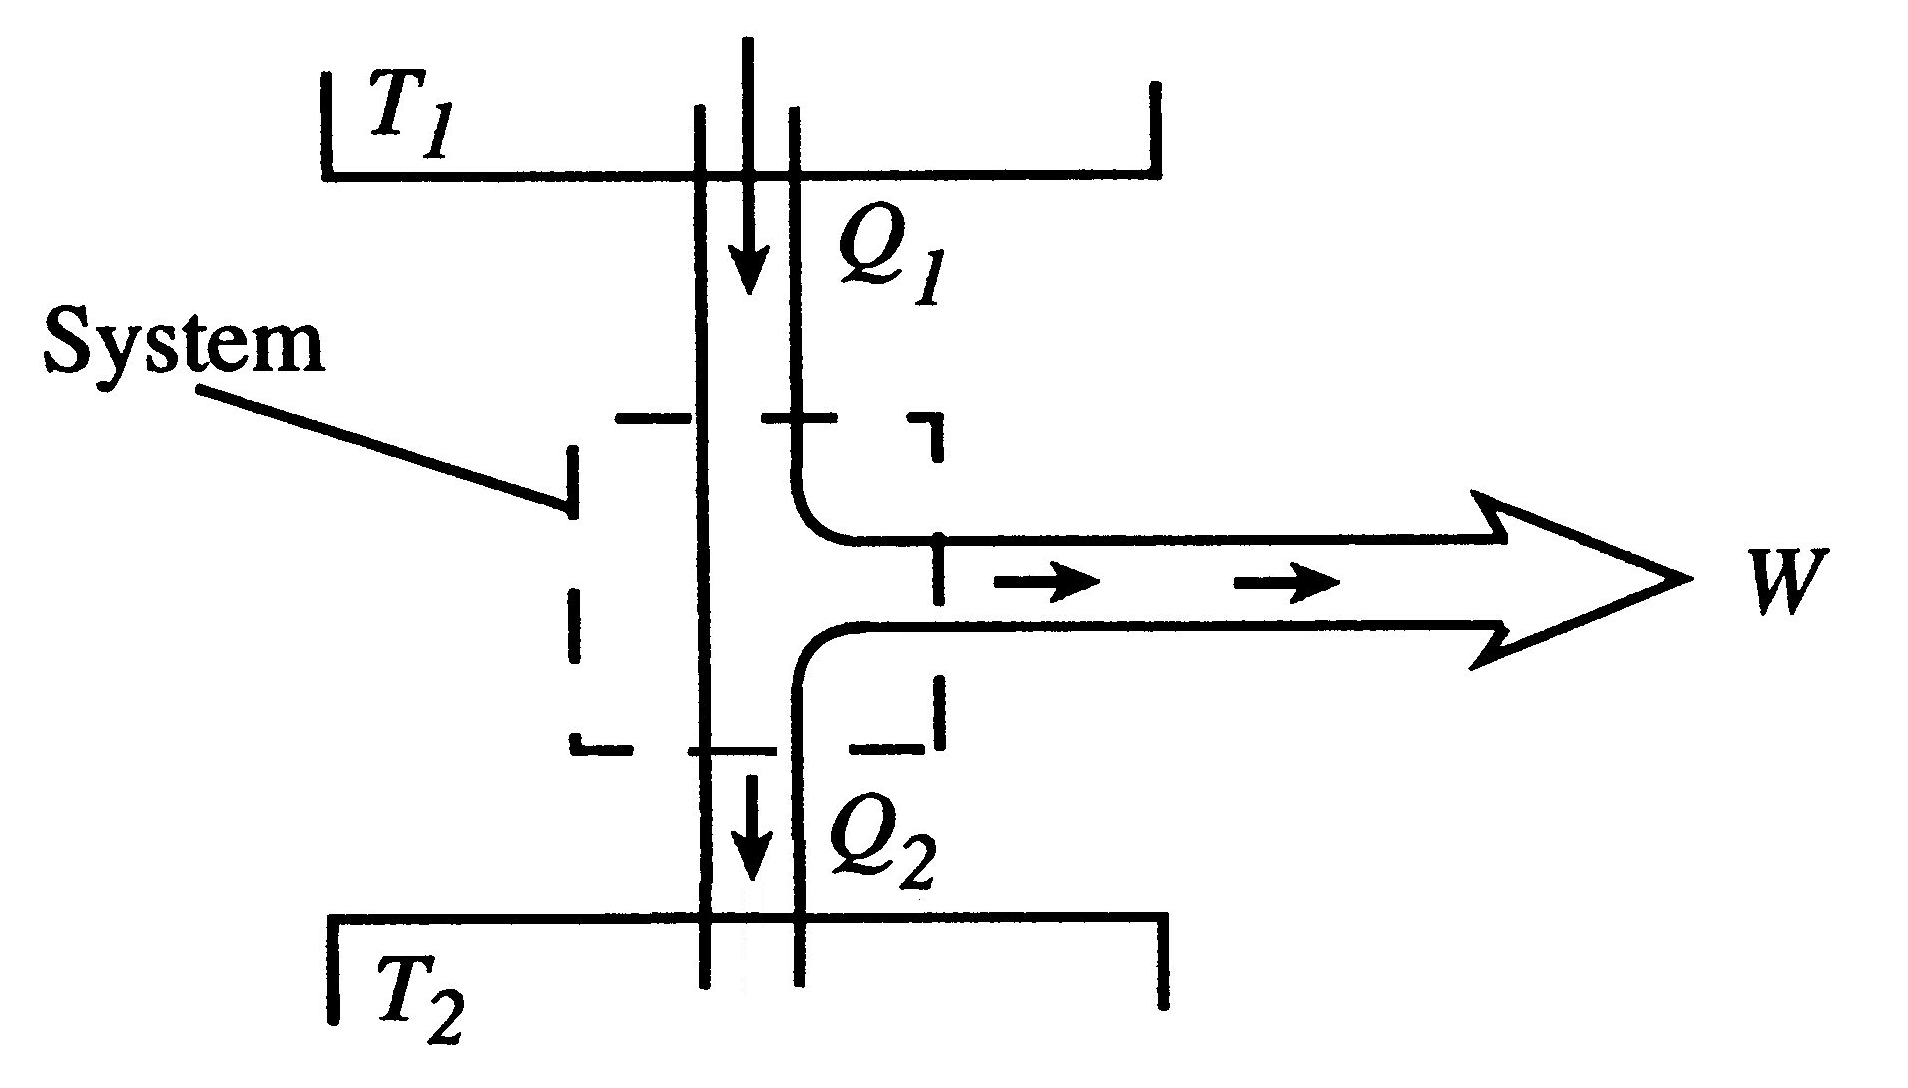
\includegraphics[width=0.4\textwidth]{second_law.png}
    \centering
    \caption{Lorem ipsum}
    \label{fig:lorem-ipsum}
\end{figure}

\lipsum[6]

\subsection{Another subsection}

\lipsum[7]

\begin{align*}
    \Delta U = W_{Point} = \int_{r_{a}}^{r_{b}} \vec{F_{Point}} \ \vec{dr}
\end{align*}    

\begin{equation}
    \Delta U = W_{Point} = - \int_{r_{a}}^{r_{b}} \vec{F_{Elec}} \ \vec{dr}
\end{equation} 

\lipsum[8]

\section{More information}

\lipsum[9-11]

\subsection{And another subsection}

\lipsum[11-13]
